In order to design the rover's camera which will be used to study rocks and to implement a robust algorithm to carry out a 3D map of the rock's surface, different characteristics of Mars and of the target need to be specified. However, as all of them cannot be taken into account, some simplifications and choices will be assumed.

\paragraph*{Mars delimitation}
~\\
Plenty of missions on Mars have been realized and a great deal of data has already been gathered. Nevertheless, even if some of them will be used to designed our system, others will be simplified or even ignored.
The first simplification concern the atmosphere of Mars. Indeed, even if its composition is now well know, it will be assumed that the dirt on the surface Mars plus the different layers of the atmosphere absorb, or scatter, 10\% of the solar energy. Moreover, the influence on the image acquisition that the dirt between the target and the camera could have will not be taken into account.
The second reduction cover the temperature. Indeed, even if it can reach -143\textdegree C during winter, 27\textdegree C during summer and have around 60\textdegree C variations between daytime and nighttime\cite{wiki:temperature}, we will assume that the CCD sensor works well all the time.

\paragraph*{Target delimitation}
~\\
Regarding the target, that is to say the part of the rock being studied, it is supposed to :
\begin{itemize}
\item be vertical;
\item not exceed 2*2 meters
\item have an area between 0.1 and 1 square meters;
\item have a relief less than  meters.
\end{itemize}

\paragraph*{Camera delimitation}
~\\
Then, regarding the camera which is designed during this study, it is presumed to :
\begin{itemize}
\item be between one and two meters far from the target;
\item be right in front of the target, that is to say that the angle between the normal of the target's surface and the focal axis of the camera is 0\textdegree;
\item be able to capture the image of a target of 2 meters height maximum.
\end{itemize}

The different characteristics of target and the camera are represented figure \ref{fig:schema system}


\begin{figure}[h]
  %\centering
  \centerline{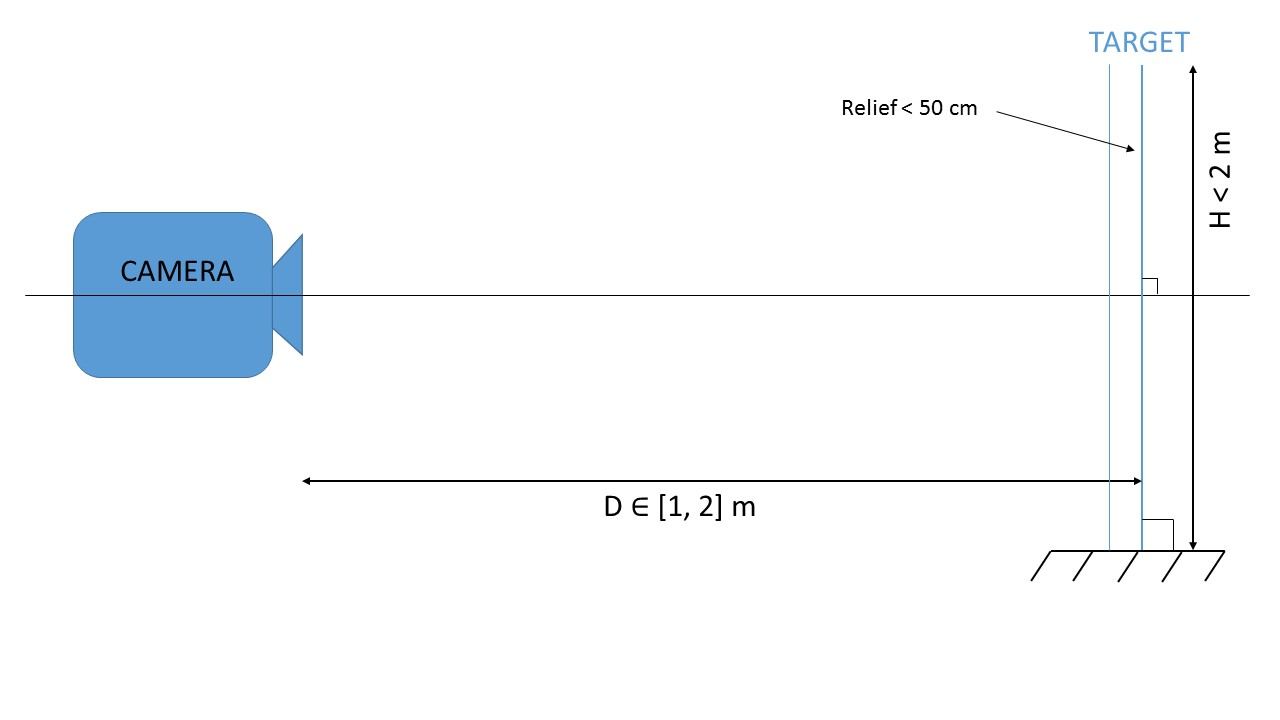
\includegraphics[scale=0.4]{fig/schemaSystem.jpg}}
  \caption{Schema of the scene}
  \label{fig:schema system}
\end{figure}

